%%%%%%%%%%%%%%%%%%%%%%%%%%%%%%%%%%%%%%%%%%%%%%%%%
%-------------Préambule-------------------------%
%%%%%%%%%%%%%%%%%%%%%%%%%%%%%%%%%%%%%%%%%%%%%%%%%

\documentclass[12pt,a4paper,twoside]{report}
\usepackage[utf8]{inputenc}
\usepackage{amsmath}
\usepackage{hyperref} %pour table des matières
\usepackage{minitoc}
\usepackage[french]{babel}
\usepackage{array,multirow,makecell} %tableau
\newcolumntype{R}[1]{>{\raggedleft\arraybackslash }b{#1}}
\newcolumntype{L}[1]{>{\raggedright\arraybackslash }b{#1}}
\newcolumntype{C}[1]{>{\centering\arraybackslash }b{#1}}
\addto\captionsfrench{\renewcommand{\chaptername}{Partie}} %Changer nom de chapitre en partie
\usepackage[Glenn]{fncychap} %pour de super titres
\usepackage{glossaries} %pour le glossaire
\makeglossaries
\usepackage[left=2cm,right=2cm,top=2cm,bottom=2cm]{geometry} %Marge
\usepackage{amsfonts}
\usepackage{amssymb}
\usepackage{textcomp} %Pour les degres celsius
%\usepackage{xcolor} %pour les couleurs
\usepackage{amsmath,amsfonts,amssymb} %mathématiques
\usepackage{graphicx}
\usepackage{caption}
\usepackage{subcaption}
\usepackage{float}
\graphicspath{{./Images/}}
\usepackage{url}

%
%
% 

\newcommand{\Surtitre}{Rapport de BE}
\newcommand{\TitreRapport}{\textbf{Introduction au Raytracing}}
\newcommand{\DateStage}{Année scolaire 2019-2020}
\newcommand{\Annee}{2020}
\newcommand{\Eleve}{Colin CROS}
\newcommand{\Professeur}{Nicolas Bonneel}
\newcommand{\Illustration}{illustration}
%
%
%

\renewcommand{\thesection}{\arabic{section}} %sections numérotées 1, 2...

\usepackage{listings}
\usepackage{color}
 
\definecolor{codegreen}{rgb}{0,0.6,0}
\definecolor{codegray}{rgb}{0.4,0.4,0.4}
\definecolor{codegraybis}{rgb}{0.6,0.6,0.6}
\definecolor{codepurple}{rgb}{0.58,0,0.82}
\definecolor{reddigits}{rgb}{0.64,0.08,0.25}
\definecolor{reddigits}{RGB}{169,17,1}
%\definecolor{backcolour}{RGB}{235,245,251}
%\definecolor{backcolour}{RGB}{253,250,254}
\definecolor{backcolour}{RGB}{250,244,254}
\definecolor{bluetitle}{RGB}{83,101,158}

\lstdefinestyle{mystyle}{
    backgroundcolor=\color{backcolour},   
    commentstyle=\color{codegraybis},
    keywordstyle=\color{blue},
    numberstyle=\color{codegray},
    stringstyle=\color{codegreen},
    basicstyle=\footnotesize,
    breakatwhitespace=false,         
    breaklines=true,                 
    captionpos=b,                    
    keepspaces=true,                 
    numbers=left,                    
    numbersep=5pt,                  
    showspaces=false,                
    showstringspaces=false,
    showtabs=false,                  
    tabsize=2,
    literate=
            {0}{{\textcolor{reddigits}{0}}}{1}
            {1}{{\textcolor{reddigits}{1}}}{1}
            {2}{{\textcolor{reddigits}{2}}}{1}
            {3}{{\textcolor{reddigits}{3}}}{1}
            {4}{{\textcolor{reddigits}{4}}}{1}
            {5}{{\textcolor{reddigits}{5}}}{1}
            {6}{{\textcolor{reddigits}{6}}}{1}
            {7}{{\textcolor{reddigits}{7}}}{1}
            {8}{{\textcolor{reddigits}{8}}}{1}
            {9}{{\textcolor{reddigits}{9}}}{1}
}
 
\lstset{style=mystyle}

\usepackage{fancyhdr} %pour un style de page personnalisé 
\pagestyle{fancy}

\renewcommand{\headrulewidth}{1pt}
\renewcommand{\footrulewidth}{1pt}
\fancyfoot[R]{\textbf{page \thepage}} 
\fancyfoot[C]{Colin CROS, École Centrale de Lyon}
\fancyfoot[L]{2019}
\fancyhead[LO]{\emph{\leftmark}}
\fancyhead[RO]{}
\fancyhead[RE]{\textit{\rightmark}}
\fancyhead[LE]{}

\begin{document}
\pagenumbering{arabic}
	

%%%%%%%%%%%%%%%%%%%%%%%%%%%%%%%%%%%%%%%%%%%%%%%%%%%%
%------------------Page de garde--------------------
%%%%%%%%%%%%%%%%%%%%%%%%%%%%%%%%%%%%%%%%%%%%%%%%%%%%

\thispagestyle{empty} %pour pas que ça numérote la page
\noindent %supprimer l'indentation


\begin{center}

	\begin{figure}[H]
	
\includegraphics[width=0.5\textwidth]{centrale_lyon}
	\end{figure}
	\vspace{5\baselineskip}
	
	\begin{center}
	{\Large \textbf{\Eleve}} \\ 
	\end{center}
	
	\vfill
	
	{\Large \textsc{\Surtitre}} \\
	\rule{9.5cm}{0.2pt} \\ %Trace trait horizontal
	\vspace{1\baselineskip} %espacement 
	{\LARGE \TitreRapport}
	\begin{figure}[H]
	\centering
	\includegraphics[width=0.8\textwidth]{\Illustration}
	\end{figure}

	
	\vfill
	\begin{table}[h!]
		\centering
		\begin{tabular}{r} %faire flotter tableau dans un environnement table colonne à 		gauche et à gauche
		\DateStage \\
		Professeur : \Professeur\\
		\end{tabular}
	\end{table}
			
\end{center}

\newpage

\newpage\section*{Introduction}

Ce rapport présente les différents rendus obtenus lors des BE du cours de Raytracing. La chronologie suivie est celle des BE. Pour chaque BE, seront présentés les méthodes implémentées et les résultats graphiques obtenus. La partie théorique ne sera pas développée.
\smallbreak
Pour les simulations, la scène utilisée sera une boite fermée par 6 sphères. Deux sphères seront présentes, une grande au centre de la scène et une seconde plus petite sur sa droite. Un triangle sera ajouté par la suite dont 2 sommets sont les centres des sphères. Les couleurs et les positions des différents objets sont illustrées dans la figure \ref{fig:be0}. Le mur situé derrière la caméra est de la même couleur que le mur en face (beige). La lumière sera placée derrière la caméra sur la gauche.

\begin{figure}[H]
	\centering
	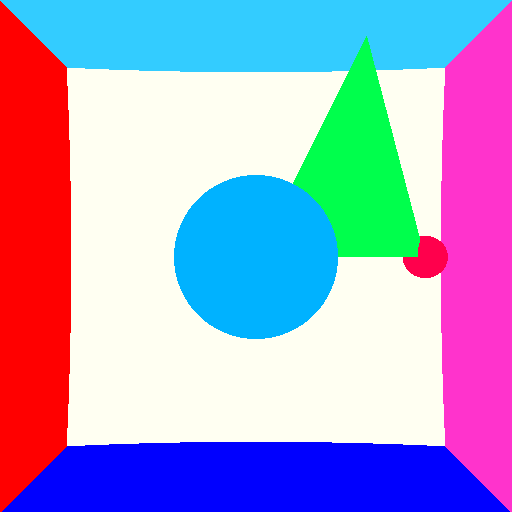
\includegraphics[width=0.45\textwidth]{be0}
	\caption{Scène sans éclairage}
	\label{fig:be0}
\end{figure}

Note : pour réaliser cette illustration pour chaque pixel, un seul rayon a été envoyé et la couleur du premier objet intersecté lui a été affectée.

A la fin du document vous trouverez comme demandé mon avis sur le cours dans sa globalité.

\newpage\section{BE 1 - Création d'une scène et éclairage}

\subsection{Création d'une scène}
Les deux premiers BE avaient pour but de créer une scène et de l'éclairer. La première étape a été de lancer des rayons depuis la caméra et de détecter des collisions avec les sphères. La figure \ref{fig:be1_01} illustre la détection d'intersection. Pour chaque pixel, un rayon est lancé dans la direction du pixel; en cas d'intersection avec une sphère le pixel est allumé (en blanc), sinon il reste noir. 

\begin{figure}[H]
	\centering
	\begin{subfigure}{.45\textwidth}
		\centering
		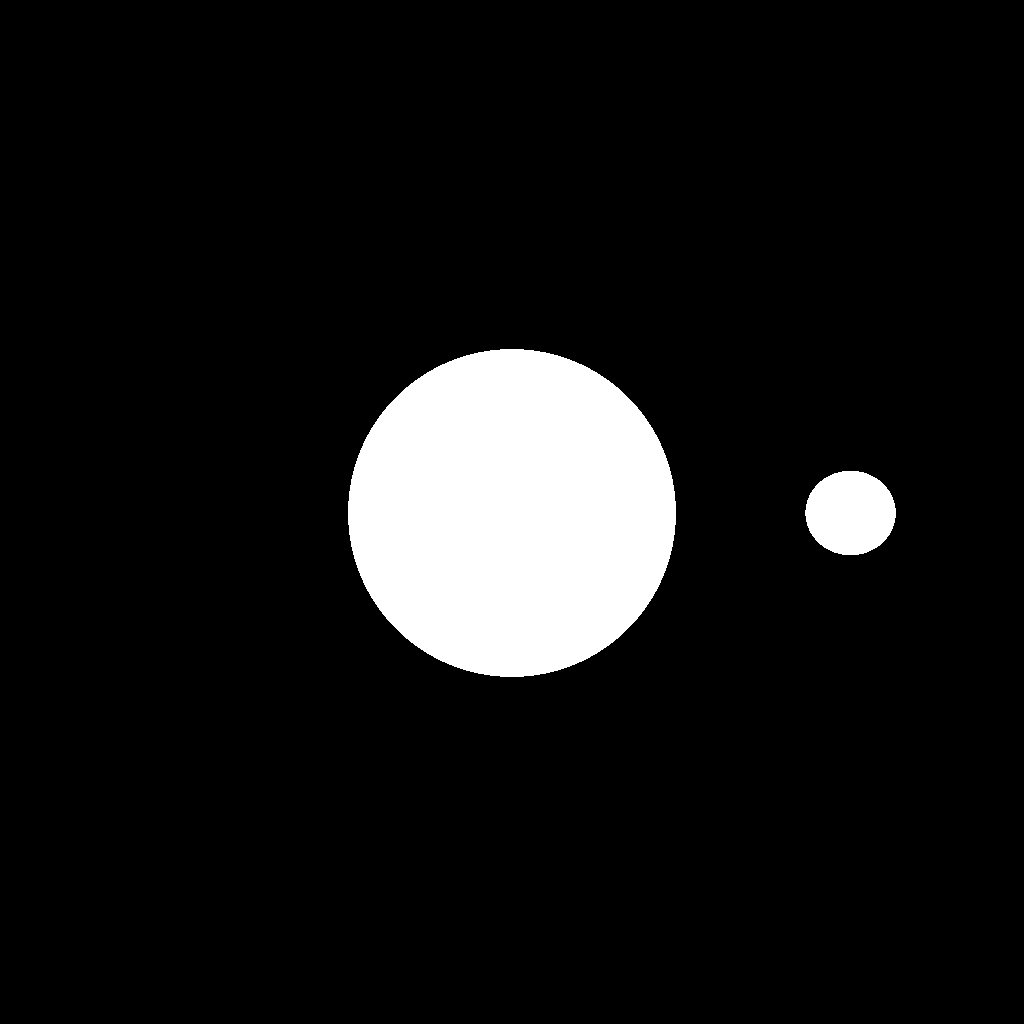
\includegraphics[width=1.\linewidth]{be1_01}
		\caption{Test d'intersection}
		\label{fig:be1_01}
	\end{subfigure}
	\begin{subfigure}{.45\textwidth}
		\centering
		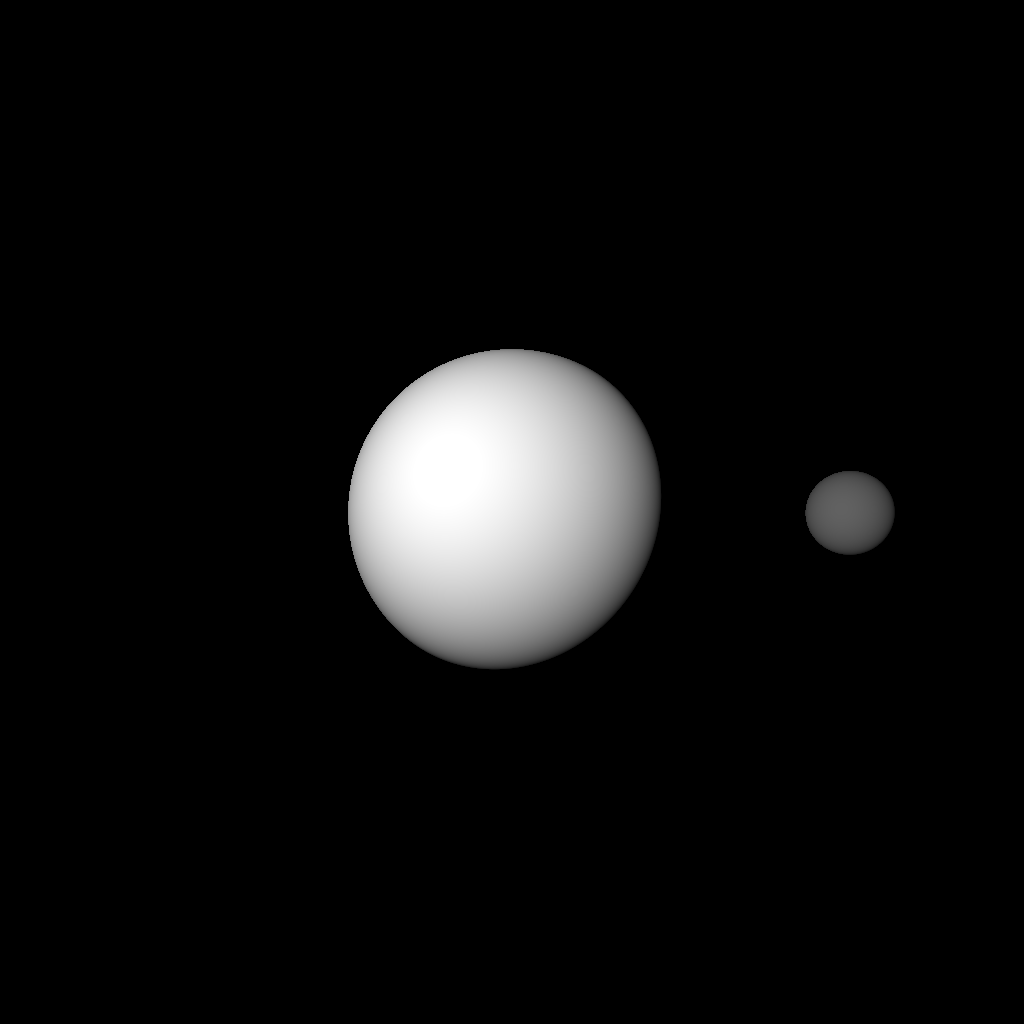
\includegraphics[width=1.\linewidth]{be1_02}
		\caption{Eclairage simple}
		\label{fig:be1_02}
	\end{subfigure}
	\caption{}
\end{figure}


L'étape suivante est l'ajout d'une lumière pour éclairer les sphères. L'intensité du pixel est calculée grâce à la formule \eqref{eq:intensite_pixel} à partir de :
\begin{itemize}
	\item la distance $d$ entre la lumière et le point d'intersection;
	\item le produit scalaire entre la normale à la sphère $\mathbf{n}$ et le vecteur unitaire pointant vers de la lumière incidente $\mathbf{u_{light}}$;
	\item l'intensité de la lumière $I_{light}$.
\end{itemize}

\begin{equation}
	\label{eq:intensite_pixel}
	I = \frac{I_{light}}{d^2}\max\left(0, \mathbf n \cdot \mathbf{u_{light}}\right)
\end{equation}

Le rendu de cet éclairage est illustré sur la figure \ref{fig:be1_02}.

\subsection{Ajout des ombres}

Sur la scène précédente, la petite sphère devrait être éclipsée par la grande. Pour ajouter les ombres, un second rayon est lancé depuis le point intersecté vers la lumière pour détecter les éventuels points d'intersection. Si un objet est détecté avant la lumière, le pixel n'est pas éclairé.

Les figures \ref{fig:be2_01} et \ref{fig:be2_02} montrent l'effet d'ombrage. Sur la figure \ref{fig:be2_01}, le rayon d'ombrage est lancé directement depuis le point d'intersection, à cause des erreurs d'arrondi des doubles, ce rayon ré-intersecte parfois la sphère, d'où les motifs noirs sur les sphères. Il faut donc déplacer légèrement l'origine du rayon d'ombrage, c'est ce qui est impléménté sur la figure \ref{fig:be2_02}.

\begin{figure}[H]
	\centering
	\begin{subfigure}{.45\textwidth}
		\centering
		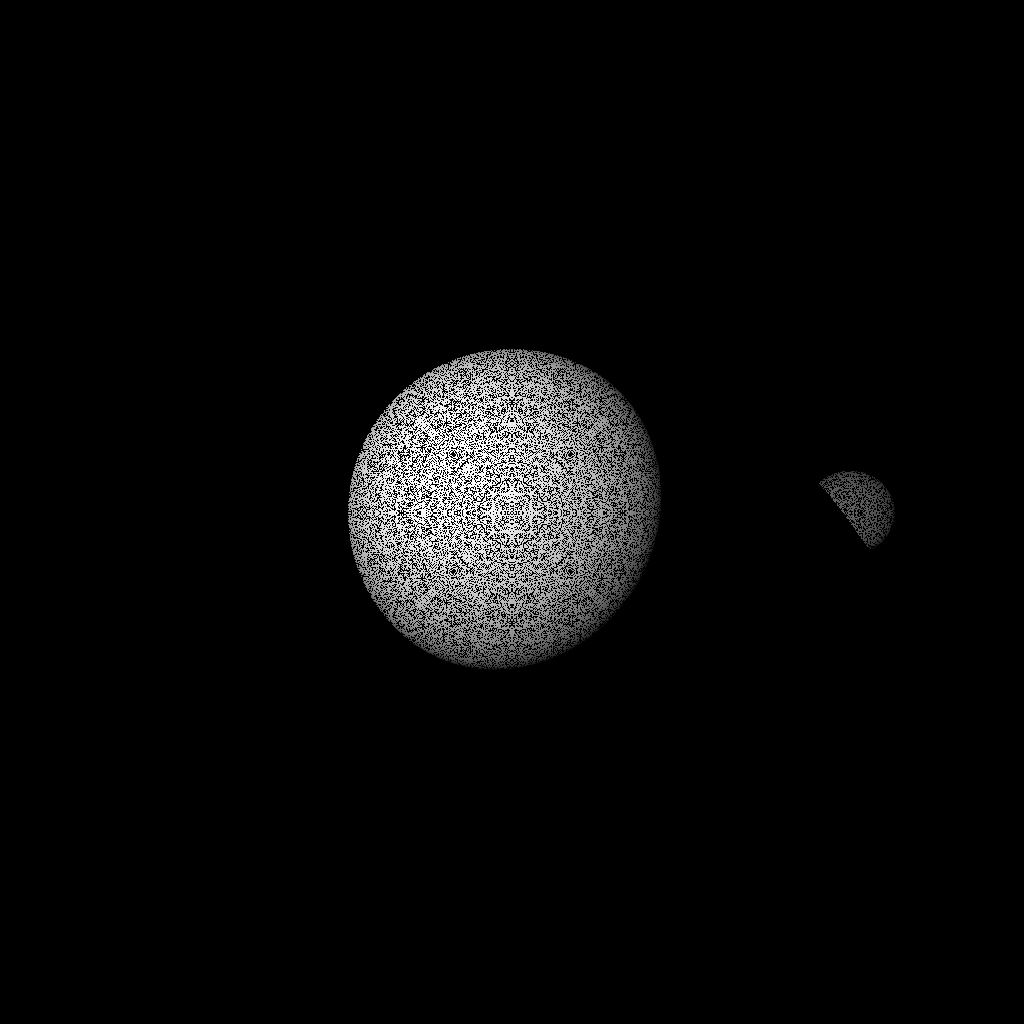
\includegraphics[width=1.\linewidth]{be2_01}
		\caption{Ombrage simple}
		\label{fig:be2_01}
	\end{subfigure}
	\begin{subfigure}{.45\textwidth}
		\centering
		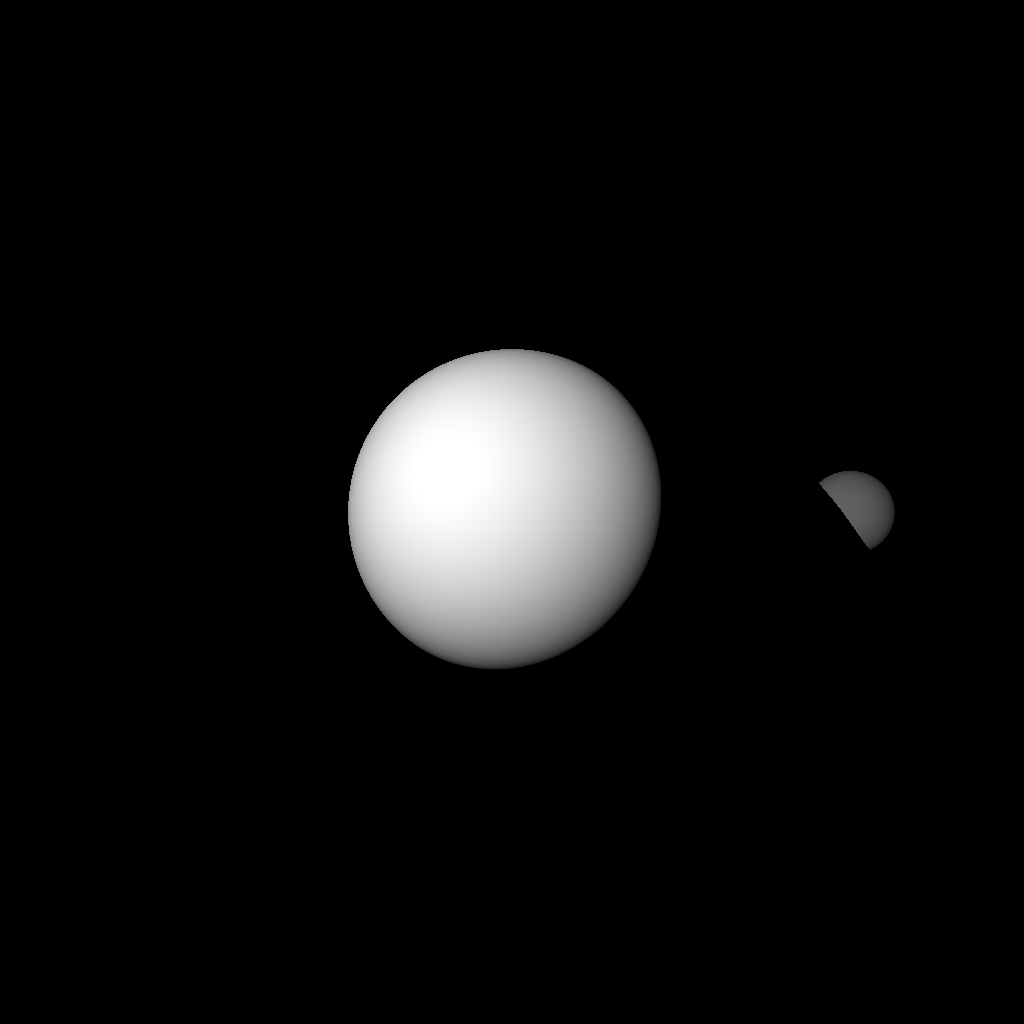
\includegraphics[width=1.\linewidth]{be2_02}
		\caption{Ombrage corrigé}
		\label{fig:be2_02}
	\end{subfigure}
	\caption{}
\end{figure}

\newpage\section{BE 2 - Matériau : couleur, miroir et transparence}
\subsection{Couleurs}
L'étape suivante est l'ajout de couleurs aux sphères. Il suffit de colorer le pixel en fonction de la couleur de la sphère. La figure \ref{fig:be2_03} reprend la scène et y ajoute des couleurs. La boite englobante présentée en introduction a également été ajoutée.

La correction gamma a aussi été implémentée. L'intensité des pixels est corrigée par la formule :
\begin{equation}
	I' = I^\frac{1}{\gamma}
\end{equation}
avec $\gamma = 2.2$. L'intensité de la lumière est également modifiée en fonction.

\begin{figure}[H]
	\centering
	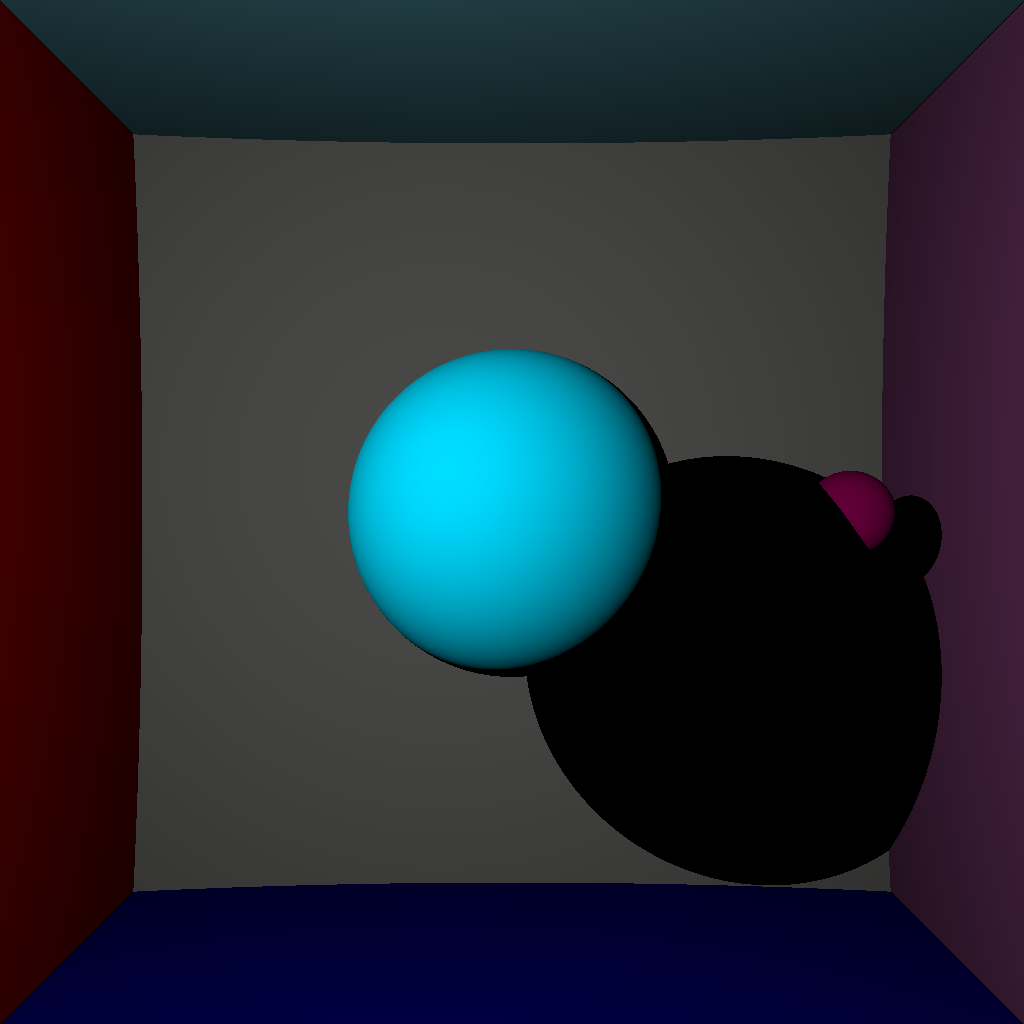
\includegraphics[width=0.45\textwidth]{be2_03}
	\caption{Scène colorée}
	\label{fig:be2_03}
\end{figure}

\subsection{Miroir}
Pour créer des surfaces miroirs, il suffit de renvoyer le rayon dans une direction symétrique par rapport à la normale. On peut même créer des miroirs colorés simplement en colorant le rayon.

Les figures \ref{fig:be2_04} et \ref{fig:be2_05} présentent le deux types de miroir : des miroirs simples pour la première (on peut notamment observer la réflexion du halo de lumière), et des miroirs colorés pour la seconde.

\begin{figure}[H]
	\centering
	\begin{subfigure}{.45\textwidth}
		\centering
		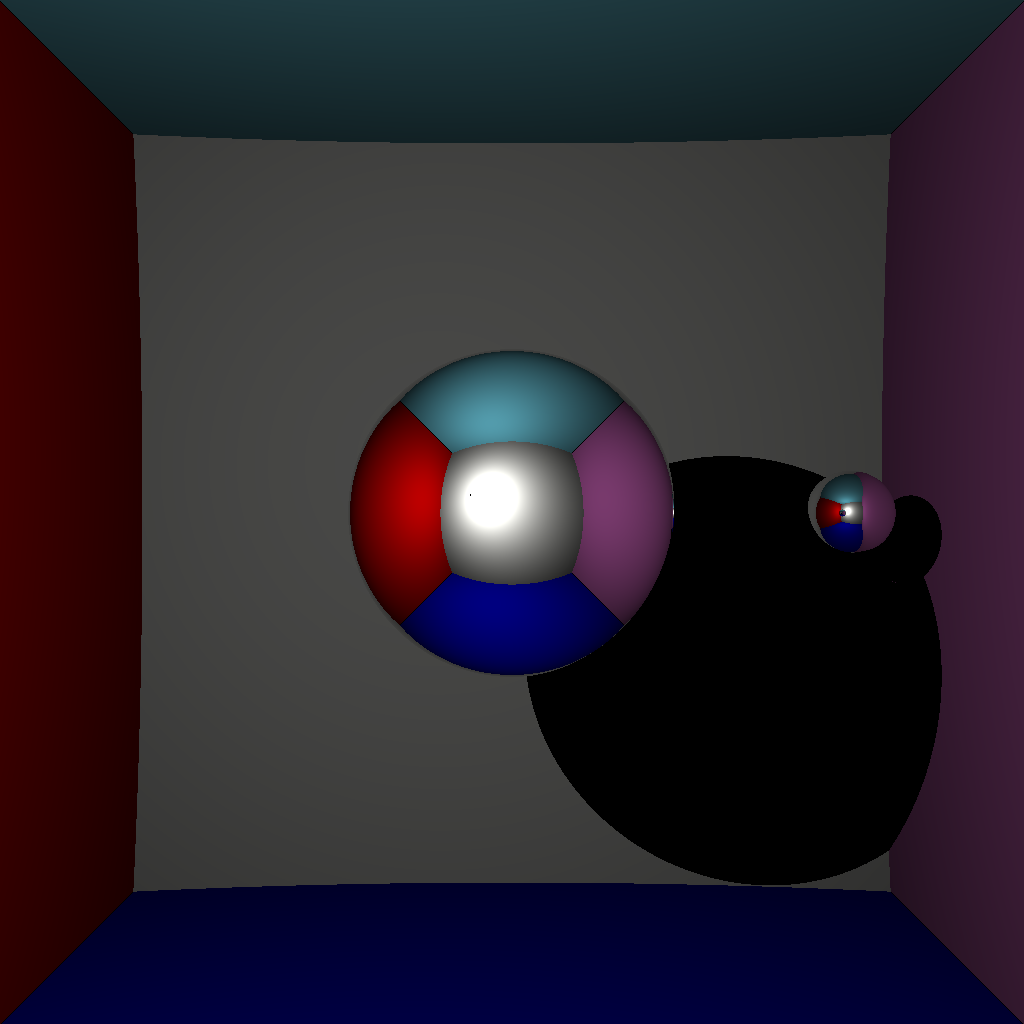
\includegraphics[width=1.\linewidth]{be2_04}
		\caption{Miroirs simples}
		\label{fig:be2_04}
	\end{subfigure}
	\begin{subfigure}{.45\textwidth}
		\centering
		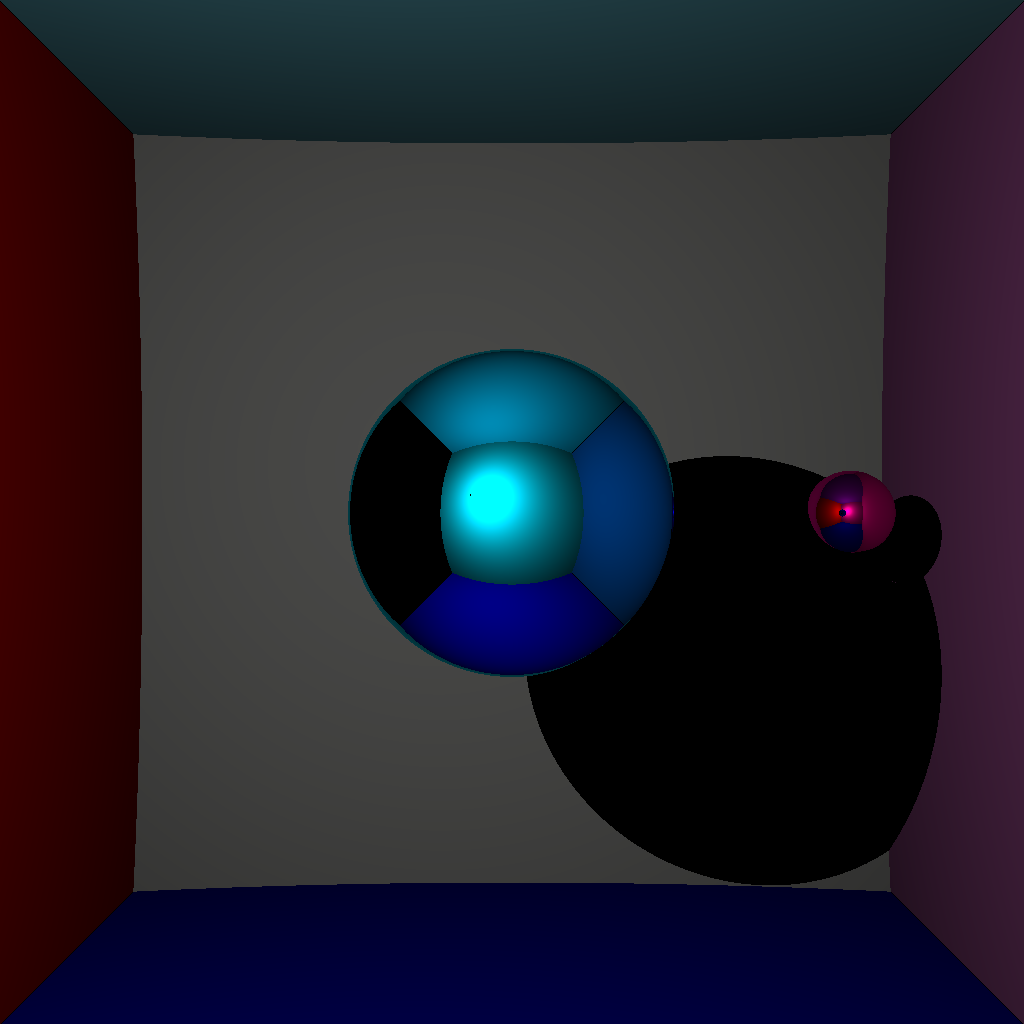
\includegraphics[width=1.\linewidth]{be2_05}
		\caption{Miroirs colorés}
		\label{fig:be2_05}
	\end{subfigure}
	\caption{}
\end{figure}

\subsection{Transparence}

Pour créer des surfaces transparentes, on implémente les lois de Snell-Descartes. La difficulté dans l'implémentation est de mémoriser si l'on se trouve à l'intérieur ou à l'extérieur d'une surface. On peut également, comme pour les miroirs, colorer les surfaces transparentes.

Les figures \ref{fig:be2_07} et \ref{fig:be2_08} illustrent la transparence avec du verre : du verre transparent pour la première, et du verre coloré pour la seconde.

\begin{figure}[H]
	\centering
	\begin{subfigure}{.45\textwidth}
		\centering
		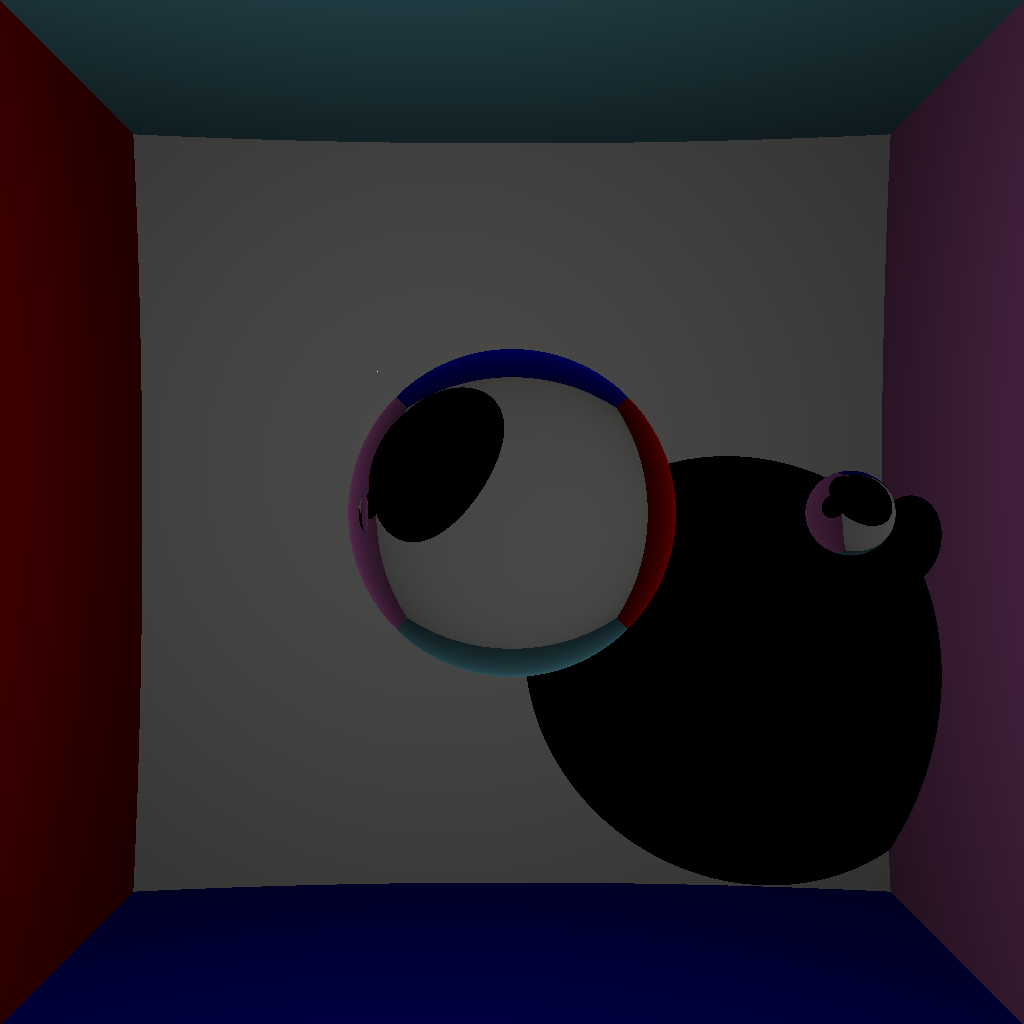
\includegraphics[width=1.\linewidth]{be2_07}
		\caption{Verres simples}
		\label{fig:be2_07}
	\end{subfigure}
	\begin{subfigure}{.45\textwidth}
		\centering
		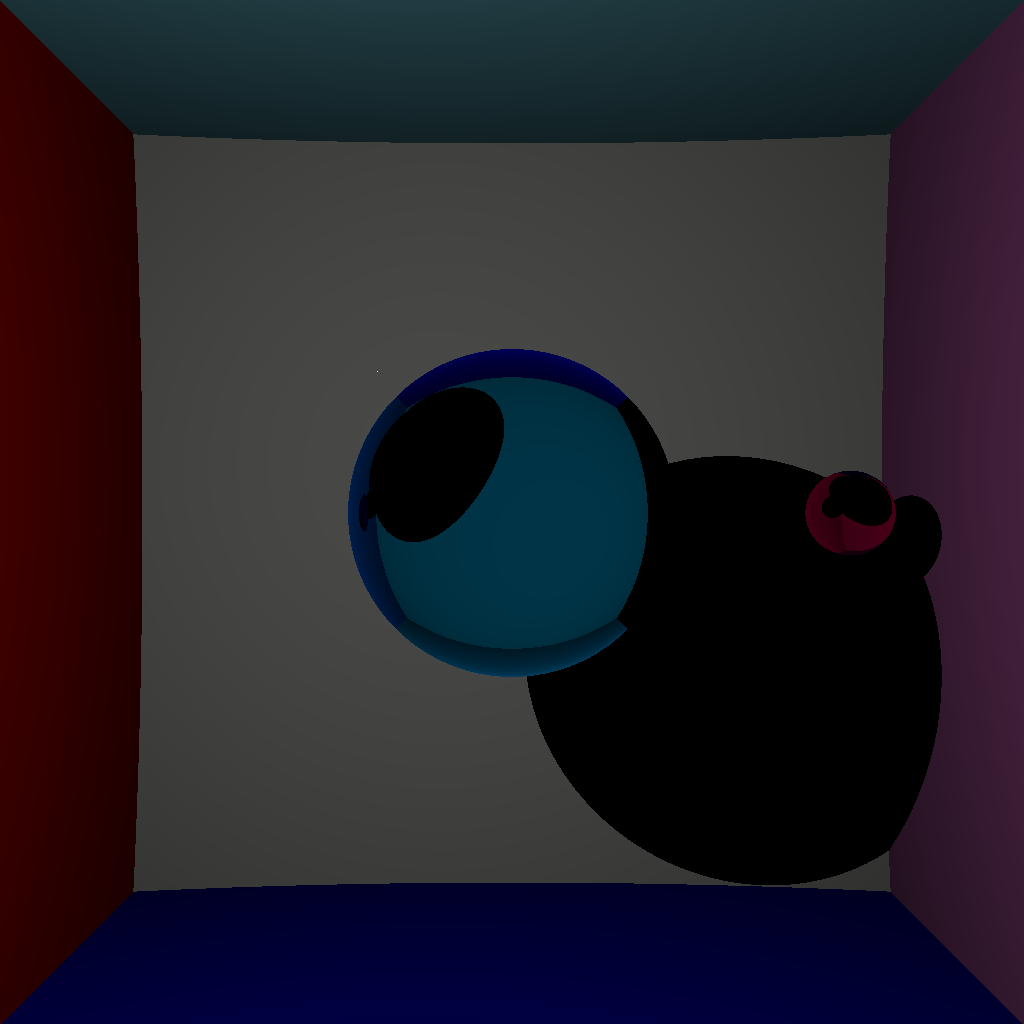
\includegraphics[width=1.\linewidth]{be2_08}
		\caption{Verres colorés}
		\label{fig:be2_08}
	\end{subfigure}
	\caption{}
\end{figure}

\newpage\section{BE 3 - Eclairage indirect et anti-crénelage}

\subsection{Eclairage indirect}

Afin d'éviter d'avoir les zones ombragées totalement noires, l'éclairage indirect est implémenté. Pour cela, lors du contact avec une sphère, on relance un rayon dans une direction aléatoire pour nuancer les couleurs. Il est nécessaire de lancer plusieurs rayons par pixel pour débruiter le rendu. La figure \ref{fig:be3_02} présente les résultats obtenus en lançant 10, 100 et 1000 rayons par pixel. On constate que plus le nombre de rayons est grand, moins l'image est bruitée.

\begin{figure}[H]
	\centering
	\begin{subfigure}{.45\textwidth}
		\centering
		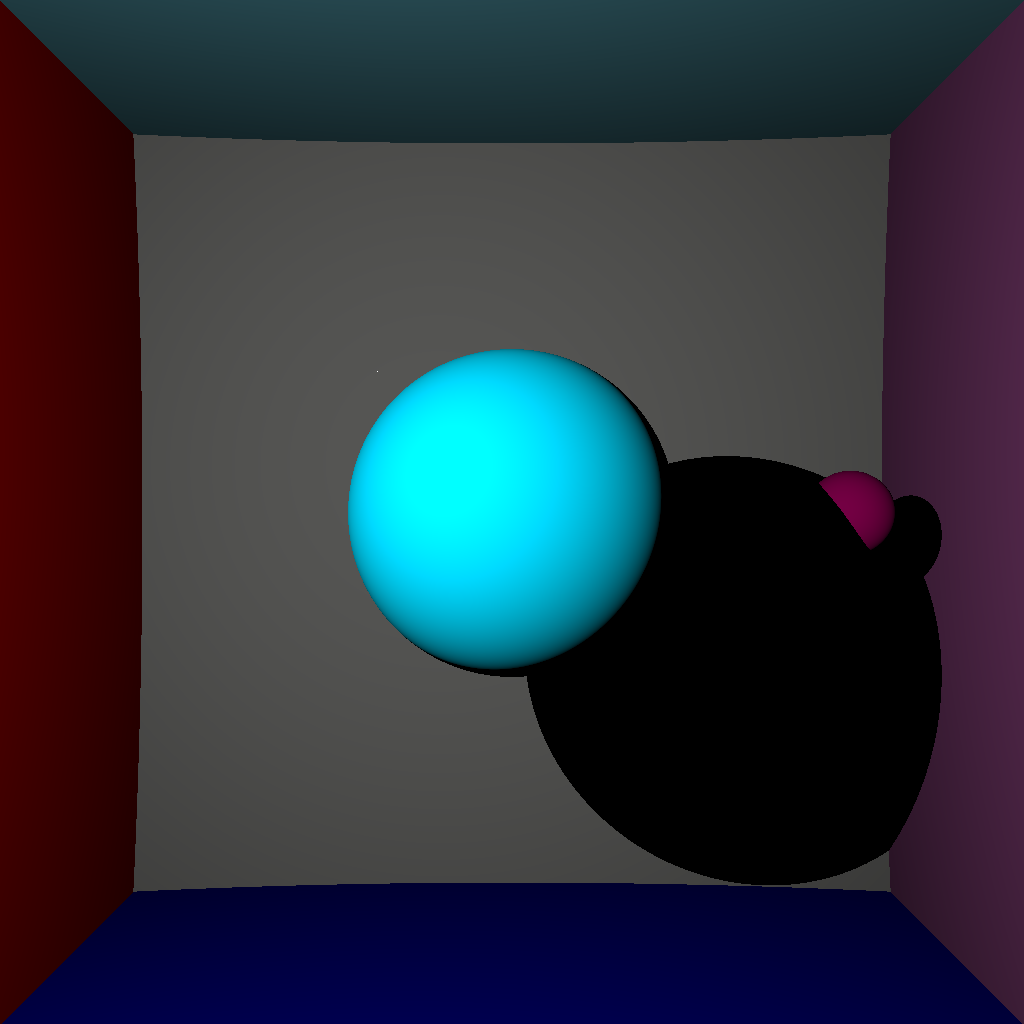
\includegraphics[width=1.\linewidth]{be3_02_1}
		\caption{Image originale}
		\label{fig:be3_02_1}
	\end{subfigure}
	\begin{subfigure}{.45\textwidth}
		\centering
		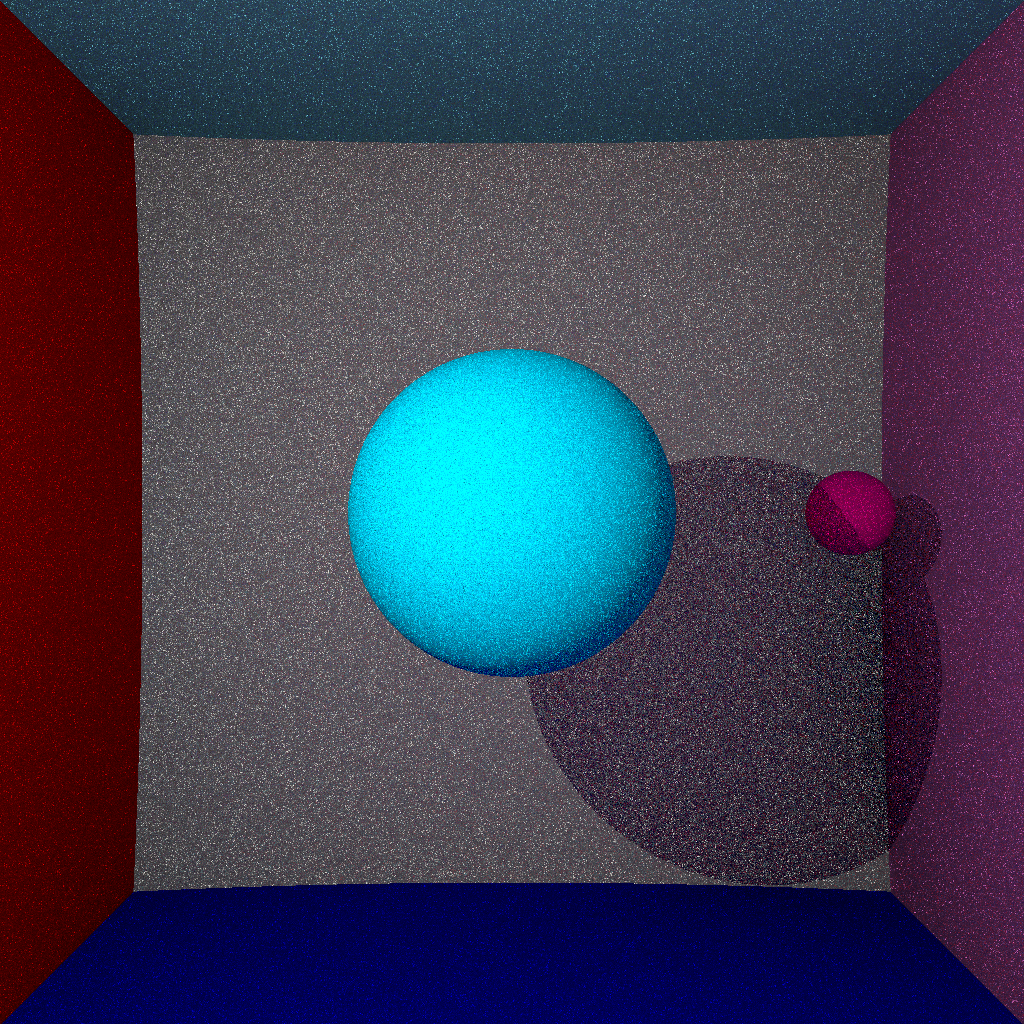
\includegraphics[width=1.\linewidth]{be3_02_10}
		\caption{10 rayons}
		\label{fig:be3_02_10}
	\end{subfigure}
	\begin{subfigure}{.45\textwidth}
		\centering
		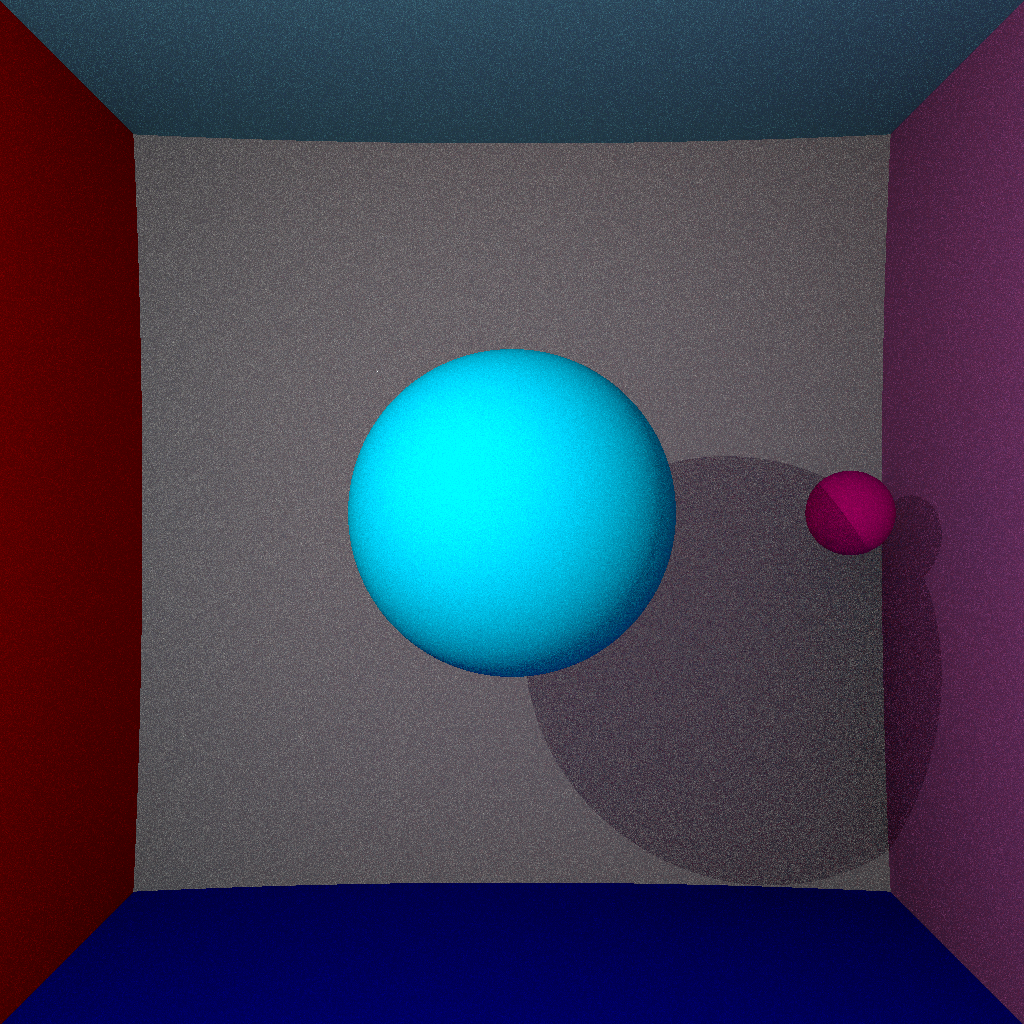
\includegraphics[width=1.\linewidth]{be3_02_100}
		\caption{100 rayons}
		\label{fig:be3_02_100}
	\end{subfigure}
	\begin{subfigure}{.45\textwidth}
		\centering
		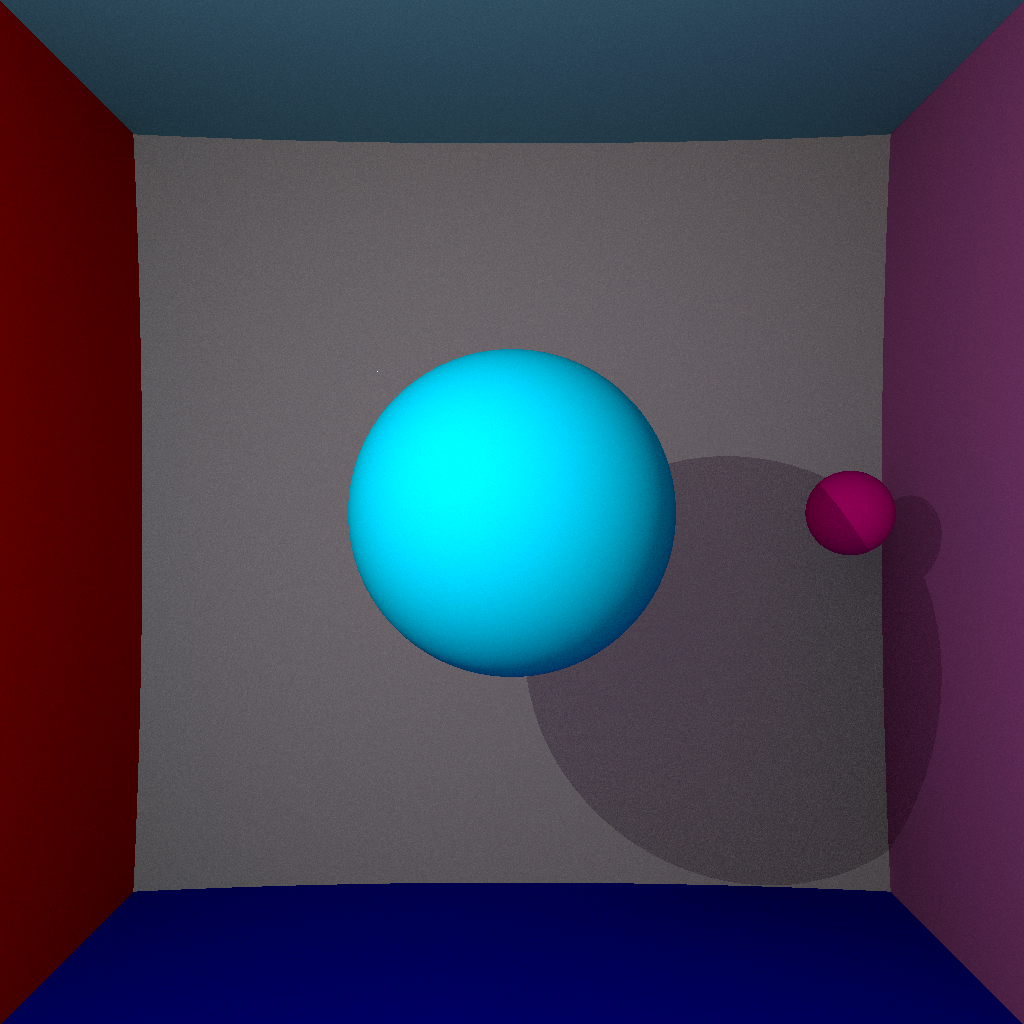
\includegraphics[width=1.\linewidth]{be3_02_1000}
		\caption{1000 rayons}
		\label{fig:be3_02_1000}
	\end{subfigure}
	\caption{Illustration de l'éclairage indirect}
	\label{fig:be3_02}
\end{figure}

\subsection{Anti-crénelage}

L'anti-crénelage permet d'éviter d'avoir une image pixelisée. A la place de lancer les rayons vers le centre du pixel considéré, on les désaxe très légèrement aléatoirement afin de lisser les contours. On ne vise plus le centre du pixel mais un point aléatoire (gaussien centré sur le centre du pixel).

Les figures \ref{fig:be3_02_1000_1} et \ref{fig:be3_03_1000_1} présentent les résultats obtenus avec et sans anti-crénelage pour 1000 rayons lancés par pixel. Un zoom a été réalisé sur la petite sphère pour que les différences soient plus marquées.

\begin{figure}[H]
	\centering
	\begin{subfigure}{.45\textwidth}
		\centering
		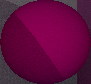
\includegraphics[width=1.\linewidth]{be3_02_1000_1}
		\caption{AC désactivé}
		\label{fig:be3_02_1000_1}
	\end{subfigure}
	\begin{subfigure}{.45\textwidth}
		\centering
		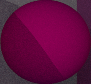
\includegraphics[width=1.\linewidth]{be3_03_1000_1}
		\caption{AC activé}
		\label{fig:be3_03_1000_1}
	\end{subfigure}
	\caption{Démonstration anti-crénelage}
\end{figure}

\newpage\section{BE 4 - Lumière diffuse et mise au point}

\subsection{Lumière diffuse}

Afin d'obtenir des ombres moins abrutes, la source de lumière ponctuelle est transformée en sphère incandescente. Plus la sphère est grande moins les ombres sont marquées. La figure \ref{fig:be4_01} présente la scène éclairée avec des lumières de différentes tailles.

\begin{figure}[H]
	\centering
	\begin{subfigure}{.45\textwidth}
		\centering
		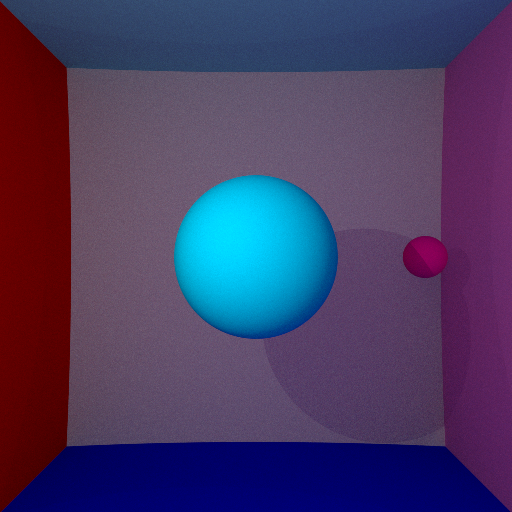
\includegraphics[width=1.\linewidth]{be4_01_1000_0}
		\caption{$R_{light} = 0.01$}
		\label{fig:be4_01_1000_0}
	\end{subfigure}
	\begin{subfigure}{.45\textwidth}
		\centering
		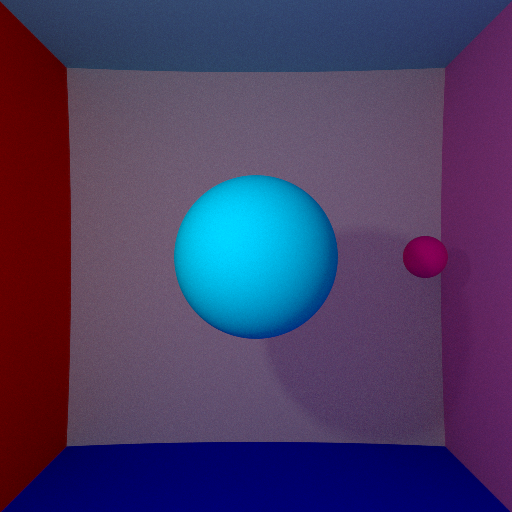
\includegraphics[width=1.\linewidth]{be4_01_1000_1}
		\caption{$R_{light} = 1$}
		\label{fig:be4_01_1000_1}
	\end{subfigure}
	\begin{subfigure}{.45\textwidth}
		\centering
		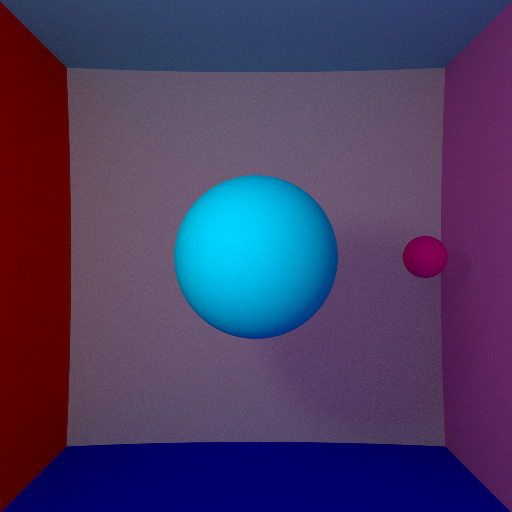
\includegraphics[width=1.\linewidth]{be4_01_1000_3}
		\caption{$R_{light} = 3$}
		\label{fig:be4_01_1000_3}
	\end{subfigure}
	\begin{subfigure}{.45\textwidth}
		\centering
		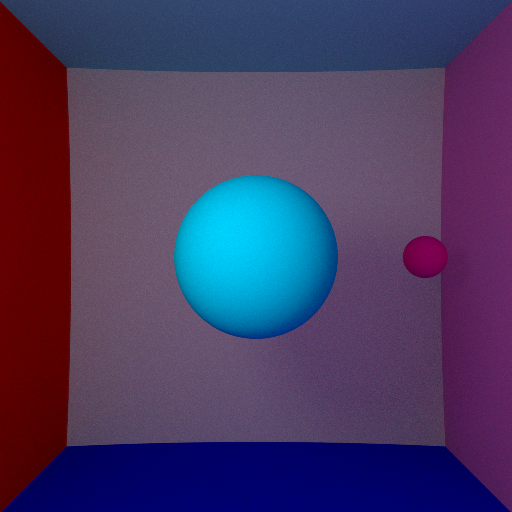
\includegraphics[width=1.\linewidth]{be4_01_1000_5}
		\caption{$R_{light} = 5$}
		\label{fig:be4_01_1000_5}
	\end{subfigure}
	\caption{Illustration de la lumière diffuse}
	\label{fig:be4_01}
\end{figure}

\subsection{Mise au point de la caméra}

Il est possible d'introduire un flou artistique comme sur les appareils photos. On introduit un angle d'ouverture plus il est grand, plus les zones en dehors de la zone de mise au point seront flous. La figure \ref{fig:be4_02} illustre ce flou artistique.

\begin{figure}[H]
	\centering
	\begin{subfigure}{.45\textwidth}
		\centering
		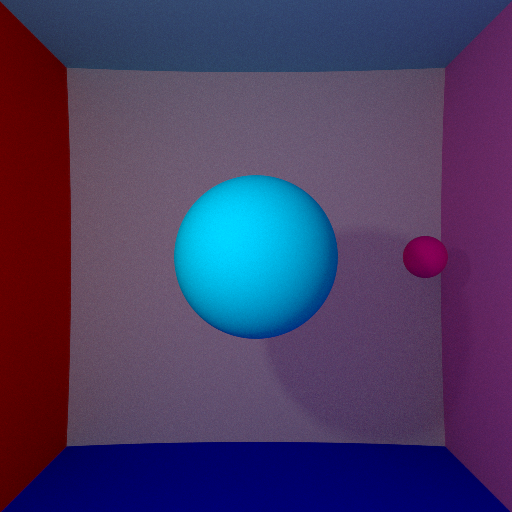
\includegraphics[width=1.\linewidth]{be4_02_1000_1_0}
		\caption{Ouverture : $0$}
		\label{fig:be4_02_1000_1_0}
	\end{subfigure}
	\begin{subfigure}{.45\textwidth}
		\centering
		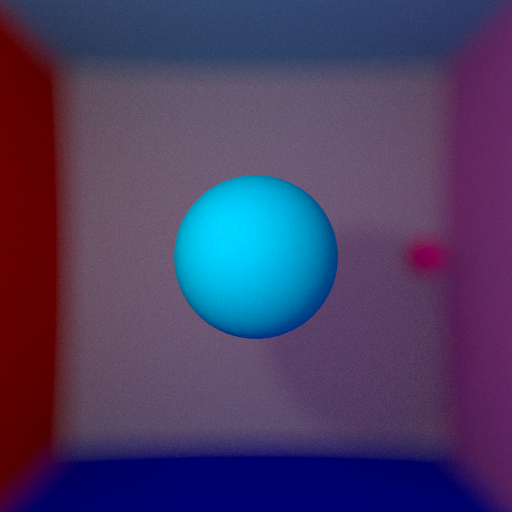
\includegraphics[width=1.\linewidth]{be4_02_1000_1_5}
		\caption{Ouverture : $5$}
		\label{fig:be4_02_1000_1_5}
	\end{subfigure}
	\caption{Démonstration ouverture}
	\label{fig:be4_02}
\end{figure}

\newpage\section{BE 5 et 6 - Les maillages et boites englobantes}

Pour afficher des maillages, il faut d'abord être capable d'afficher un triangle. La figure \ref{fig:be5_01_100R} démontre que l'affichage d'un triangle fonctionne correctement.

Ensuite, on peut afficher des \emph{models} générés à partir de maillage. Dans un premier temps, ils ne sont pas texturés comme le montre la figure \ref{fig:be6_01_100R_5O}.

\begin{figure}[H]
	\centering
	\begin{subfigure}{.45\textwidth}
		\centering
		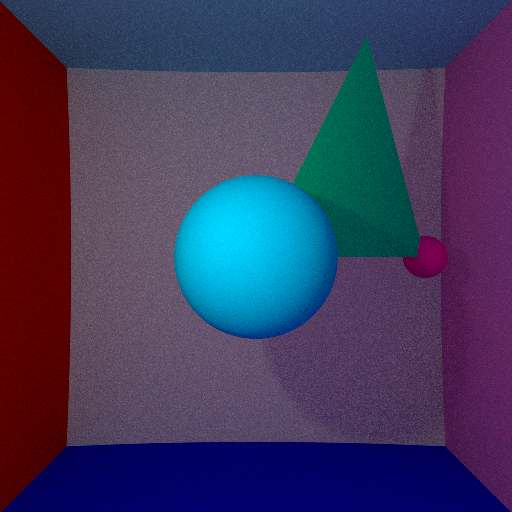
\includegraphics[width=1.\linewidth]{be5_01_100R}
		\caption{Affichage d'un triangle}
		\label{fig:be5_01_100R}
	\end{subfigure}
	\begin{subfigure}{.45\textwidth}
		\centering
		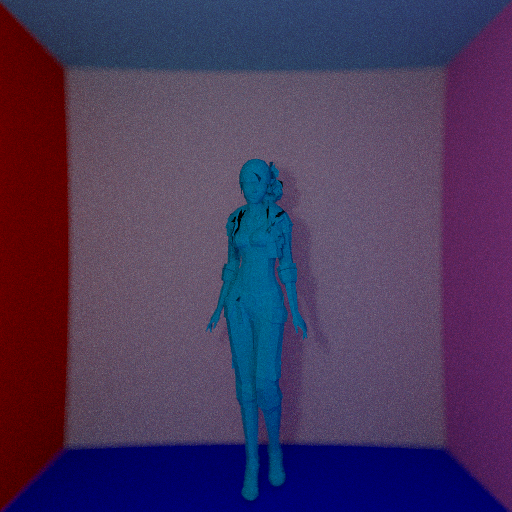
\includegraphics[width=1.\linewidth]{be6_01_100R_5O_75s}
		\caption{Affichage d'un maillage}
		\label{fig:be6_01_100R_5O}
	\end{subfigure}
\end{figure}

Afin d'accélérer les calculs, on réalise une arborescence de boites englobantes. Pour 100 rayons par pixel, la génération de la figure \ref{fig:be6_01_100R_5O} prenait environ 1 minute 15 sans les boites contre une dizaine de secondes avec.

Enfin pour avoir des maillages moins cubique, on lisse grâce aux coordonnées barycentriques les normales. Les figures \ref{fig:be6_01_100R_5O_1} et \ref{fig:be6_02_100R_5O} illustrent ce lissage.

\begin{figure}[H]
	\centering
	\begin{subfigure}{.45\textwidth}
		\centering
		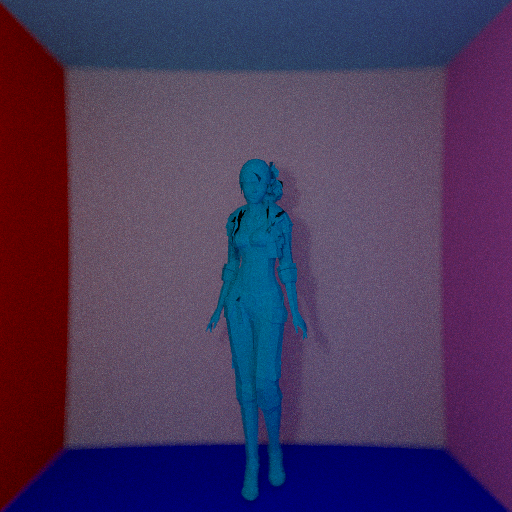
\includegraphics[width=1.\linewidth]{be6_01_100R_5O_75s}
		\caption{Sans lissage}
		\label{fig:be6_01_100R_5O_1}
	\end{subfigure}
	\begin{subfigure}{.45\textwidth}
		\centering
		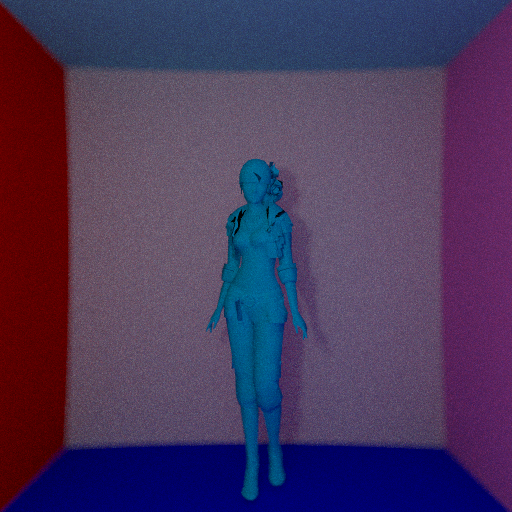
\includegraphics[width=1.\linewidth]{be6_02_100R_5O}
		\caption{Avec lissage}
		\label{fig:be6_02_100R_5O}
	\end{subfigure}
	\caption{Illustration du lissage des normales}
\end{figure}

\newpage\section{BE 7 - Texture et effet plastique}

\subsection{Ajout des textures}

Pour donner de la couleur aux maillages on ajoute des textures. Les textures sont ajoutées en utilisant les coordonnées UV. La figure \ref{fig:be7_01_100R_5O} reprend le modèle précédent en le coloriant.

\subsection{Effet plastique}

On ajoute pour finir de la brillance en décomposant la BRDF en 2 termes : le terme de diffusion classique et un terme de réfléchissant. Cela génère un effet \emph{glossy} sur les objets comme le montre la figure \ref{fig:be7_03_1000R_5O_10000n}.

\begin{figure}[H]
	\centering
	\begin{subfigure}{.45\textwidth}
		\centering
		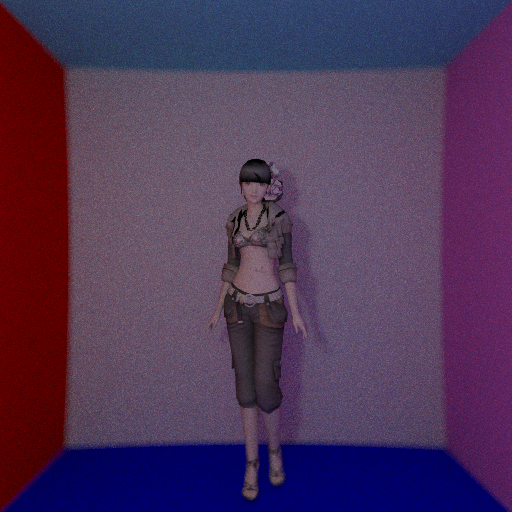
\includegraphics[width=1.\textwidth]{be7_01_100R_5O}
		\caption{Modèle coloré "matte" (100 rayons)}
		\label{fig:be7_01_100R_5O}
		\end{subfigure}
	\begin{subfigure}{.45\textwidth}
		\centering
		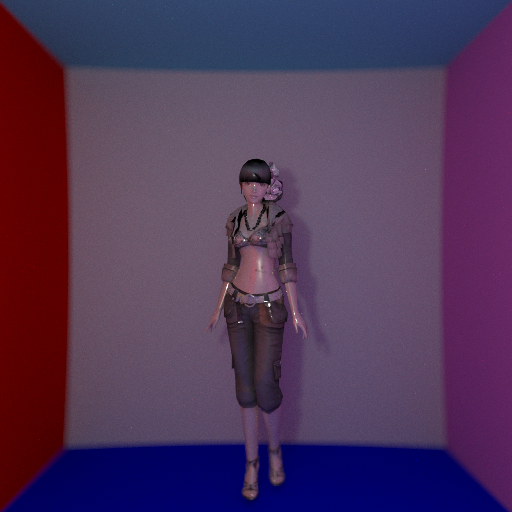
\includegraphics[width=1.\textwidth]{be7_03_1000R_5O_10000n}
		\caption{Modèle coloré "glossy" (1000 rayons)}
		\label{fig:be7_03_1000R_5O_10000n}
	\end{subfigure}
	\caption{}
\end{figure}

\newpage
\section{Bonus : réalisation de l'illustration de titre}

Pour réaliser l'illustration de la page de garde (figure \ref{fig:illustration}), deux éléments ont été ajoutés :
\begin{itemize}
	\item un pavage en damier sur les triangle;
	\item une texturisation UV des sphères.
\end{itemize}
La boite cubique a été créée à partir de triangles (deux par face). Deux miroirs triangulaires légèrement colorés ont été placés aux deux coins inférieurs ainsi qu'une balle avec effet plastique. La tache noire dans le miroir gauche correspond à la lumière.

\begin{figure}[H]
	\centering
	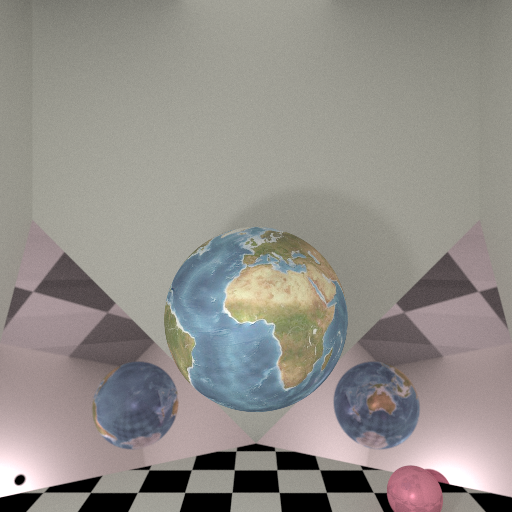
\includegraphics[width=0.80\textwidth]{illustration}
	\caption{Scène bonus}
	\label{fig:illustration}
\end{figure}

\subsection{Pavage en damier}

Pour réaliser un pavage en damier, une classe triangle pavé a hérité de la classe triangle. La seule différence vient du calcul de la couleur, on peut lui affecter deux couleurs selon la valeur de la fonction $f(P ; h)$ avec
\begin{itemize}
	\item $P(x,y,z)$ le point auquel on calcule la couleur ;
	\item $h$ le pas du dallage ;
	\item $f(P ; h) = \left(\lfloor x/h\rfloor + \lfloor y/h\rfloor +\lfloor z/h\rfloor\right)\%2$.
\end{itemize}
Un pas de $10$ a été utilisé pour le sol et de $40$ pour le plafond (visible dans les miroirs).

\subsection{Texturisation des sphères}

Pour ajouter la texture de la Terre, les coordonnées UV sont utilisées. La texture a été téléchargée sur Google et une fonction inspirée de la méthode d'ajout de texture du maillage a été implémentée.

Les coordonnées UV sur une sphère unitaire et centrée sur l'origine s'obtiennent grâce aux formules ci-dessous :
\begin{align}
	U &= \frac{1}{2\pi}\left(\pi + \arctan(x/z)\right)\\
	V &= \frac{1}{\pi}\left(\pi - \arccos(y)\right)
\end{align}

\newpage
\section*{Remarque sur le cours}
\vfill
Personnellement, j'ai beaucoup apprécié ce cours, en particulier le fait d'avoir tout implémenté et de ne pas avoir utilisé de bibliothèque préconstruite. Je pense poursuivre les vidéos pour voir ce qui vient après l'effet glossy.
\vspace{1cm}

J'avais déjà fait un peu de C++ en stage, donc je n'ai pas été dérangé par le langage. Je pense qu'il faudrait tout de même indiquer dans le fascicule de cours que le C++ est un pré-requis pour ce module. Au niveau de la charge de travail, je suis venu à tous les cours et je pense y avoir consacré environ 2h supplémentaires par semaine en moyenne à l'exception du BE sur la lumière indirecte où j'ai eu énormément d'erreurs, les vidéos m'ont permis de me remettre à jour pour le cours suivant.
\vspace{1cm}

J'ai aimé le format du cours en mode BE-cours, le rythme me semblait bon. Les vidéos apportent un réel plus quand on décroche et ne sont pas trop redondantes avec le cours. J'en ai regardé certaines après le cours, et c'était intéressant parce qu'à plusieurs reprises, je n'ai pas implémenté de la même manière que vous (parfois j'aurais dû...).
\vspace{1cm}

Au niveau des points d'amélioration du cours, je n'ai rien à redire, je ne savais pas trop à quoi m'attendre et je n'ai pas été déçu.
\vfill
PS : on n'avait rien contre vous, on prend toujours un café à 10h.

\end{document}



